\section{Introduction}
\dropcap{I}mitation Learning \citep{schaal1999imitation, zare2024survey} has regained substantial traction in recent years due to its superior sample and iteration efficiency in acquiring complex tasks compared to Reinforcement Learning. Recent work has focused on improving the robustness, expressiveness, and generalization of motion policies learned from demonstration by leveraging modern ML architectures such as diffusion models and flow matching~\citep{chi2023diffusion, black2024pi0}; scaling up the number of demonstrations to increase robustness~\citep{o2024open, black2024pi0, gemini2025robotics}; training across multiple robot embodiments (e.g., different manipulators) to promote generalization~\citep{o2024open, black2024pi0}; and conditioning policies on semantic task instructions and environment context via embeddings from large \glspl{VLM}~\citep{black2024pi0, gemini2025robotics}.
Among these, \glspl{DMP}~\citep{ijspeert2002learning, ijspeert2013dynamical, saveriano2023dynamic, hu2024fusion} parametrize a motion policy through dynamical systems that predict the desired velocity or acceleration based on the system’s current state. By grounding the formulation in dynamical systems, researchers can leverage established tools from nonlinear system theory~\citep{khalil2002nonlinear} to analyze and ensure-by-design convergence properties in motion primitive—such as global asymptotic stability~\citep{kober2009learning, ijspeert2013dynamical, rana2020euclideanizing, urain2020imitationflow, zhang2022learning, perez2023stable, perez2024puma} or orbital stability~\citep{ijspeert2002learning, kober2009learning, wensing2017sparse, urain2020imitationflow, khadivar2021learning, abu2021periodic, abu2024learning, zhi2024teaching, nah2025combining}. This is not typically the case for other ML-based motion policies like RNNs or Diffusion Policies (DPs)~\citep{chi2023diffusion, o2024open, black2024pi0, gemini2025robotics}.
Such approaches—often referred to as \glspl{SMP}—are robust to perturbations, disturbances, and model mismatches, as the motion policy continuously steers the system back to the desired reference. This also enhances data efficiency, a trait that is increasingly important as robots take on a broader range of tasks.

An important subclass of \gls{DMP} strategies addresses tasks that require continuous, non-resting motion—those for which rest-to-rest trajectories are neither representative nor sufficient. Canonical examples include wiping a surface, swimming, or walking, where motion generation must produce sustained activity across cycles. These so-called rhythmic or periodic \glspl{DMP} have spurred extensive research, both within the traditional dynamical systems formulation~\citep{ijspeert2002learning,kober2009learning,ijspeert2013dynamical,wensing2017sparse,kramberger2018passivity,saveriano2023dynamic,abu2024learning,hu2024fusion,nah2025combining} and in more recent methods combining simple latent-space limit cycles with learned diffeomorphic mappings~\citep{urain2020imitationflow,khadivar2021learning,zhi2024teaching}. Still, despite these advances, existing approaches struggle to reproduce non-trivial trajectories—especially those with sharp transitions, high curvature, or discontinuous velocity profiles, which are common in real-world rhythmic tasks. Overcoming this typically requires many demonstrations, thus strongly limiting their applicability in practical settings. 

Such limitations are exacerbated by the incapability of classical deterministic \glspl{DMP} to generalize across tasks~\citep{jaquier2025transfer}: a fresh or fine-tuned model must be trained for every new motion or task \citep{saveriano2023dynamic}. Although several studies have introduced task-conditioned variants—such as conditioning on encoded visual observations~\citep{bahl2020neural, mohammadi2024extended} or adopting probabilistic \glspl{DMP} formulations~\citep{seker2019conditional, saveriano2023dynamic, pekmezci2024coupled}—these methods often yield incoherent trajectories when presented with tasks they did not explicitly encounter during training~\citep{jaquier2025transfer}, even when those tasks lie within the original training distribution. 

So, despite their promise of being an alternative to data-intensive learning strategies, \glspl{DMP} ultimately require a substantial amount of data and a complex training process when tasks are varied and trajectories are not straightforward. Instead, the ability to generate purposeful motions in zero-shot settings for unseen tasks will be essential on the path towards truly generalist autonomous robots in the future.

In this paper, we introduce \glspl{OSMP}, a framework, visualized in Fig.~\ref{fig:osmp:concept_overview}, designed to address the limitations of existing rhythmic motion primitives by learning an expressive, orbitally stable limit cycle capable of capturing elaborate periodic behaviors. Our approach imposes a dynamic inductive bias by shaping the latent space according to a supercritical Hopf bifurcation oscillator; a well-studied system in nonlinear dynamics~\citep{strogatz2018nonlinear, khadivar2021learning, nah2025combining} that has remained unexplored in the context of machine learning. This core dynamical prior is complemented by a novel bijective Euclideanizing-flow encoder, extending the Real NVP architecture~\citep{rana2020euclideanizing, dinh2017density}.

Under mild architectural assumptions, we prove \glspl{OSMP} are almost-globally transverse contracting, so every trajectory converges exponentially—not merely asymptotically—to the learned limit cycle. A tailored loss suite binds the cycle’s shape and speed to the demonstration, eliminating the long-standing mismatch between a stable latent orbit and a highly curved, nonlinear sample. Thus, a single demonstration already yields an effective policy, drastically outperforming the data efficiency of DPs~\citep{chi2023diffusion}. 
A novel conditioning–interpolation loss then drives smooth, zero-shot transitions between related tasks: for example, the model continuously morphs between reverse and forward turtle-swimming gaits after seeing only those two exemplars. This ability sharply reduces the need to densely sample the motion task space and further increases data efficiency. 
We also introduce solutions for synchronizing multiple primitives in their phase and, without retraining, affinely scale, translate, or otherwise modulate the learned velocity field, turning rhythmic \glspl{DMP} into a practical, data-efficient controller for complex robots.

We rigorously validate our approach in both simulation and on hardware. Quantitative and qualitative benchmarks compare it with classical neural models (\glspl{MLP}, \glspl{RNN}, \glspl{NODE}), state-of-the-art motion policies like \gls{DP}~\citep{chi2023diffusion}, and diffeomorphic-encoder methods with stable latent dynamics, including Imitation Flow (iFlow)~\citep{urain2020imitationflow} and \gls{SPDT}~\citep{zhi2024teaching}. Experiments show our \glspl{OSMP} accurately track periodic trajectories on diverse robotic platforms—UR5 and Kuka arms, the Helix soft robot, and a hybrid underwater “crush turtle” robot. Expressed as autonomous dynamical systems, they deliver more compliant, natural behavior than time-indexed, error-based controllers. We further demonstrate in both simulations and real-world experiments in-phase synchronization of multiple \glspl{OSMP} and, via encoder conditioning, smooth interpolation among several distinct motion tasks with a single motion policy.

\begin{figure}[h!]
    \centering
    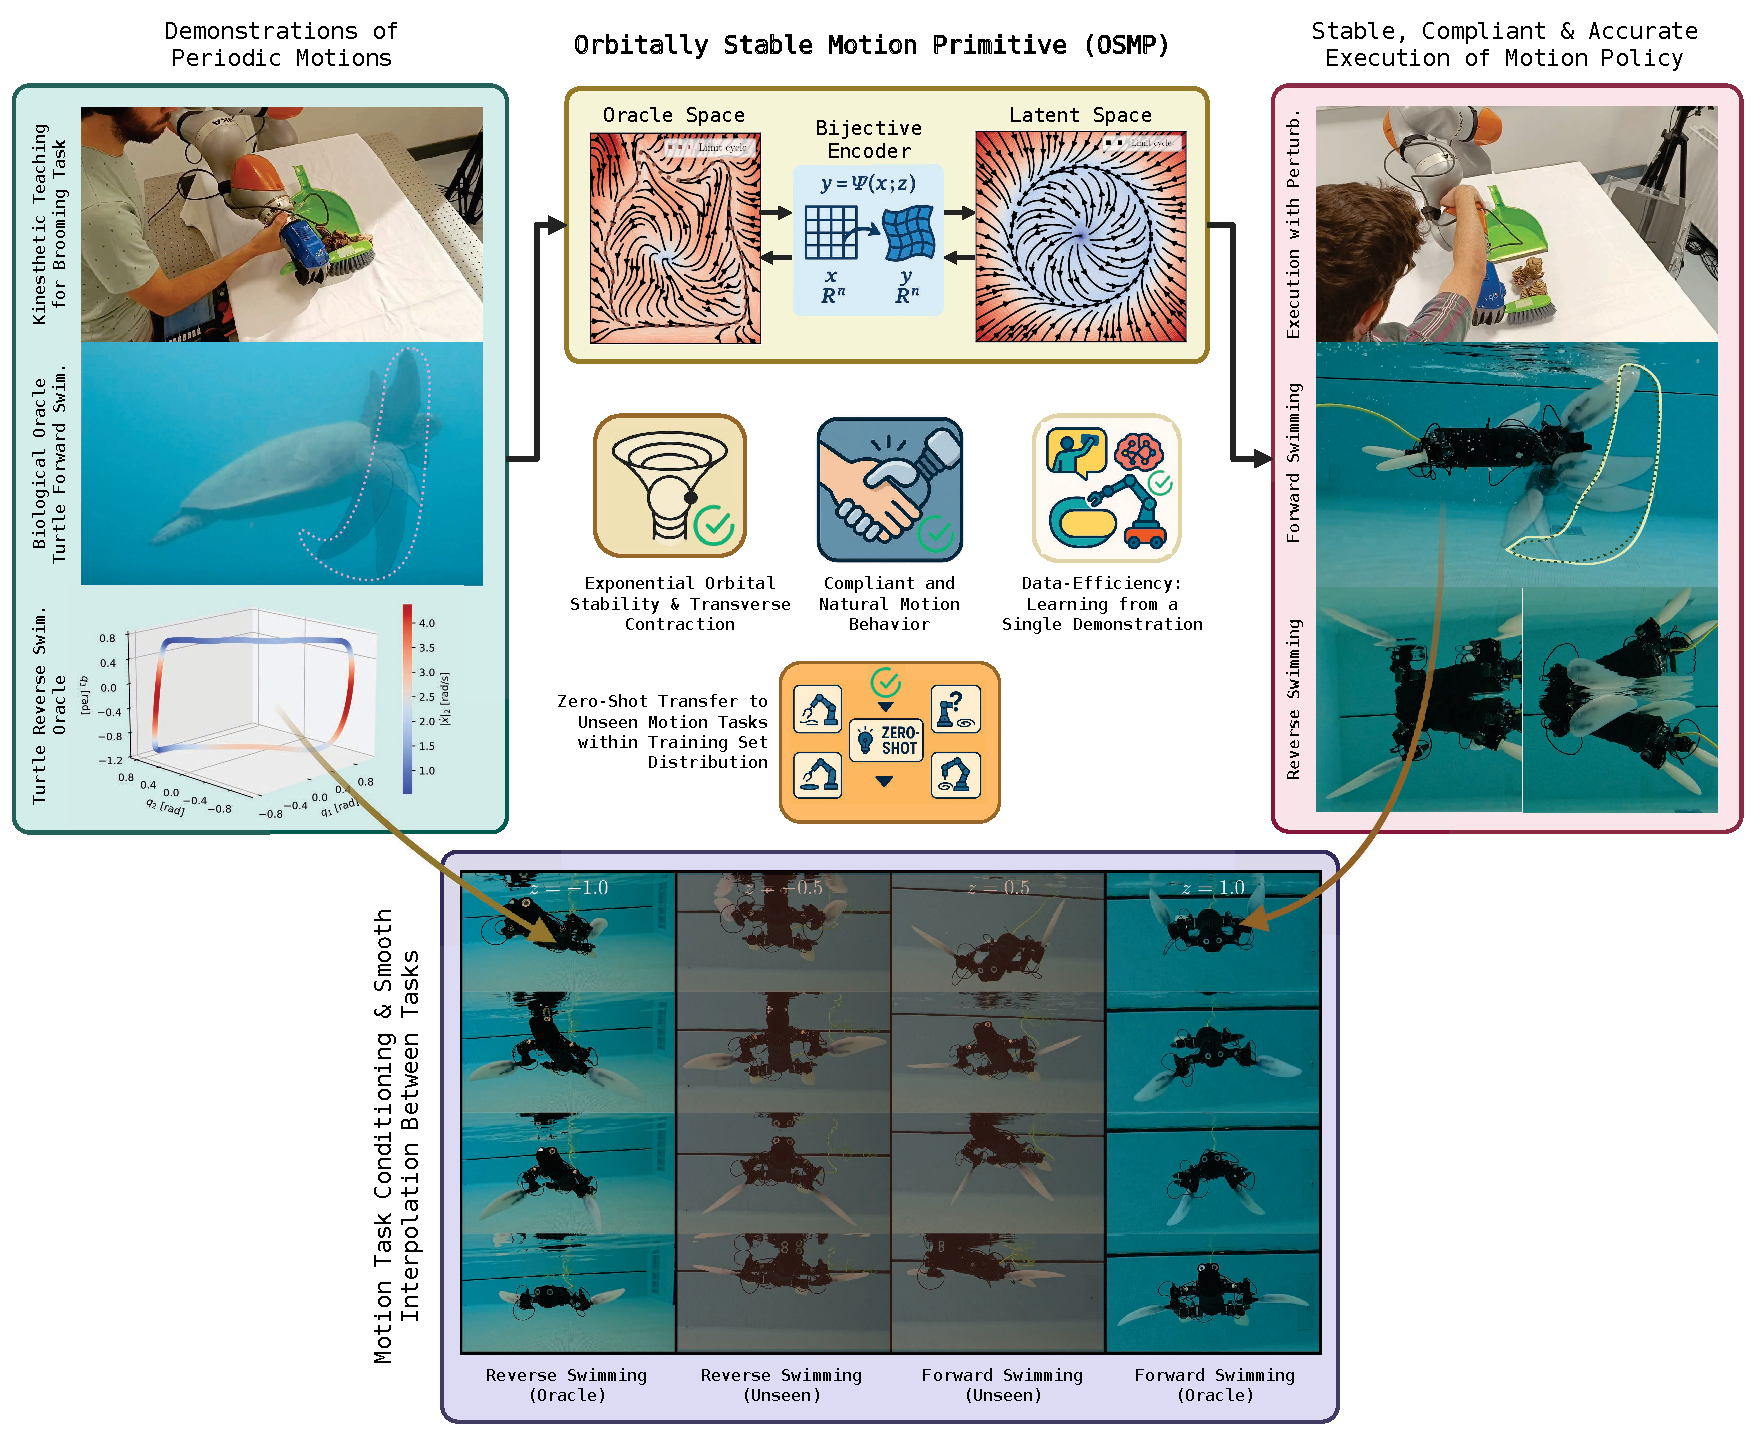
\includegraphics[width=1.0\linewidth]{osmp/figures/concept_overview/concept_overview_v1_compressed.pdf}
    % \includesvg[width=1.0\linewidth]{figures/methodology_overview/osmp_methodology_overview_v2.svg}
    \caption{
    \textbf{Overview of Features and Characteristics of \glspl{OSMP}.}
    OSMPs enable the learning of periodic motions from demonstrations while guaranteeing exponential orbital stability \& transverse contraction, instilling compliant and natural motion behavior, and outstanding data efficiency as they are able to learn complex motion behaviors from just one demonstration. Furthermore, a motion task conditioning allows the same motion policy to exhibit multiple distinct behaviors while a specially crafted loss term encourages smooth interpolation between motion tasks seen during training leading to meaningful motion behaviors on task unseen during training (i.e., zero-shot transfer).
    }
    \label{fig:osmp:concept_overview}
\end{figure}


\subsection{Methodology in a Nutshell}
Below, we provide a brief overview of the \gls{OSMP} methodology and architecture, as depicted in Fig.\ref{fig:osmp:methodology_overview}. Further details are provided in Sec.~\ref{sec:osmp:methodology}. In the \gls{DMP} framework, an \gls{OSMP} outputs the desired system velocity as $\dot{x}=f(x; z)$, with $x\in\mathbb{R}^n$ the configuration and $z$ the motion-task conditioning. The computation proceeds in three steps: (i) map $x$ into a latent coordinate $y\in\mathbb{R}^n$ using a $z$-conditioned bijective encoder (a learned diffeomorphism); (ii) evaluate the designed latent dynamics to obtain $\dot{y}$; and (iii) project $\dot{y}$ back to the original space via the encoder’s inverse Jacobian. While the architecture can be trained under various regimes (e.g., reinforcement learning), this paper focuses on imitation learning—specifically, behavior cloning—where both the latent representation y and the predicted velocity $\dot{x}$ are supervised.

\subsection{Related Work}
While there is a long history of research on both discrete and rhythmic/periodic \glspl{DMP}~\citep{ijspeert2002learning, kober2009learning, ijspeert2013dynamical, wensing2017sparse, kramberger2018passivity, saveriano2023dynamic, abu2024learning, hu2024fusion, nah2025combining}, the expressive power of classical \glspl{DMP}~\citep{ijspeert2002learning, kober2009learning, ijspeert2013dynamical, wensing2017sparse} is limited, preventing them from learning highly complex and intricate trajectories.

Recently, however, an exciting research direction has emerged that combines diffeomorphisms into a latent space—learned using ML techniques—with relatively simple, analytically tractable (e.g., linear) latent space dynamics to enhance expressiveness while preserving stability and convergence guarantees~\citep{rana2020euclideanizing, urain2020imitationflow, zhang2022learning, perez2023stable}. Most of these works focus on point-to-point motions and aim to ensure global asymptotic stability~\citep{rana2020euclideanizing, zhang2022learning, perez2023stable, perez2024puma}, although there have also been several works combining diffeomorphic encoders with rhythmic latent dynamics for learning periodic motions from demonstration~\citep{urain2020imitationflow, khadivar2021learning, zhi2024teaching}.
However, in the existing methods, either the chosen architecture for the bijective encoder lacks expressiveness~\citep{urain2020imitationflow, khadivar2021learning}, the method training is very sensitive to the initial neural network parameter~\citep{urain2020imitationflow}, the method does not learn the demonstrated velocities but only the general direction of motion~\citep{zhi2024teaching}, or cannot accurately learn very complex oracle shapes~\citep{zhi2024teaching}.

Although the proposed model architecture is similar to that of \citet{zhi2024teaching}, our training pipeline differs substantially: we incorporate an imitation loss that teaches the model the demonstrated velocities, replace the Hausdorff-distance objective with a limit-cycle matching loss better suited to complex or discontinuous paths, optionally guide latent polar angles with a time-alignment term to capture highly curved, possibly concave, contours, and regularize workspace velocities outside the demonstration to improve numerical stability during inference. 
Finally, we allow a parametrization of the polar angular velocity with a neural network, allowing the learning of complex velocity profiles along the limit cycle without compromising the strong contraction guarantees. 

Furthermore, the above-mentioned methods do not offer solutions for many practical issues, such as synchronizing multiple systems—a common requirement in locomotion or bimanual manipulation~\citep{gams2015accelerating}—or to shape the learned velocity online.

We provide a comparison with relevant existing methods in Table~\ref{tab:osmp:osmp_characteristics_vs_baselines}.

\begin{figure}[h!]
    \centering
    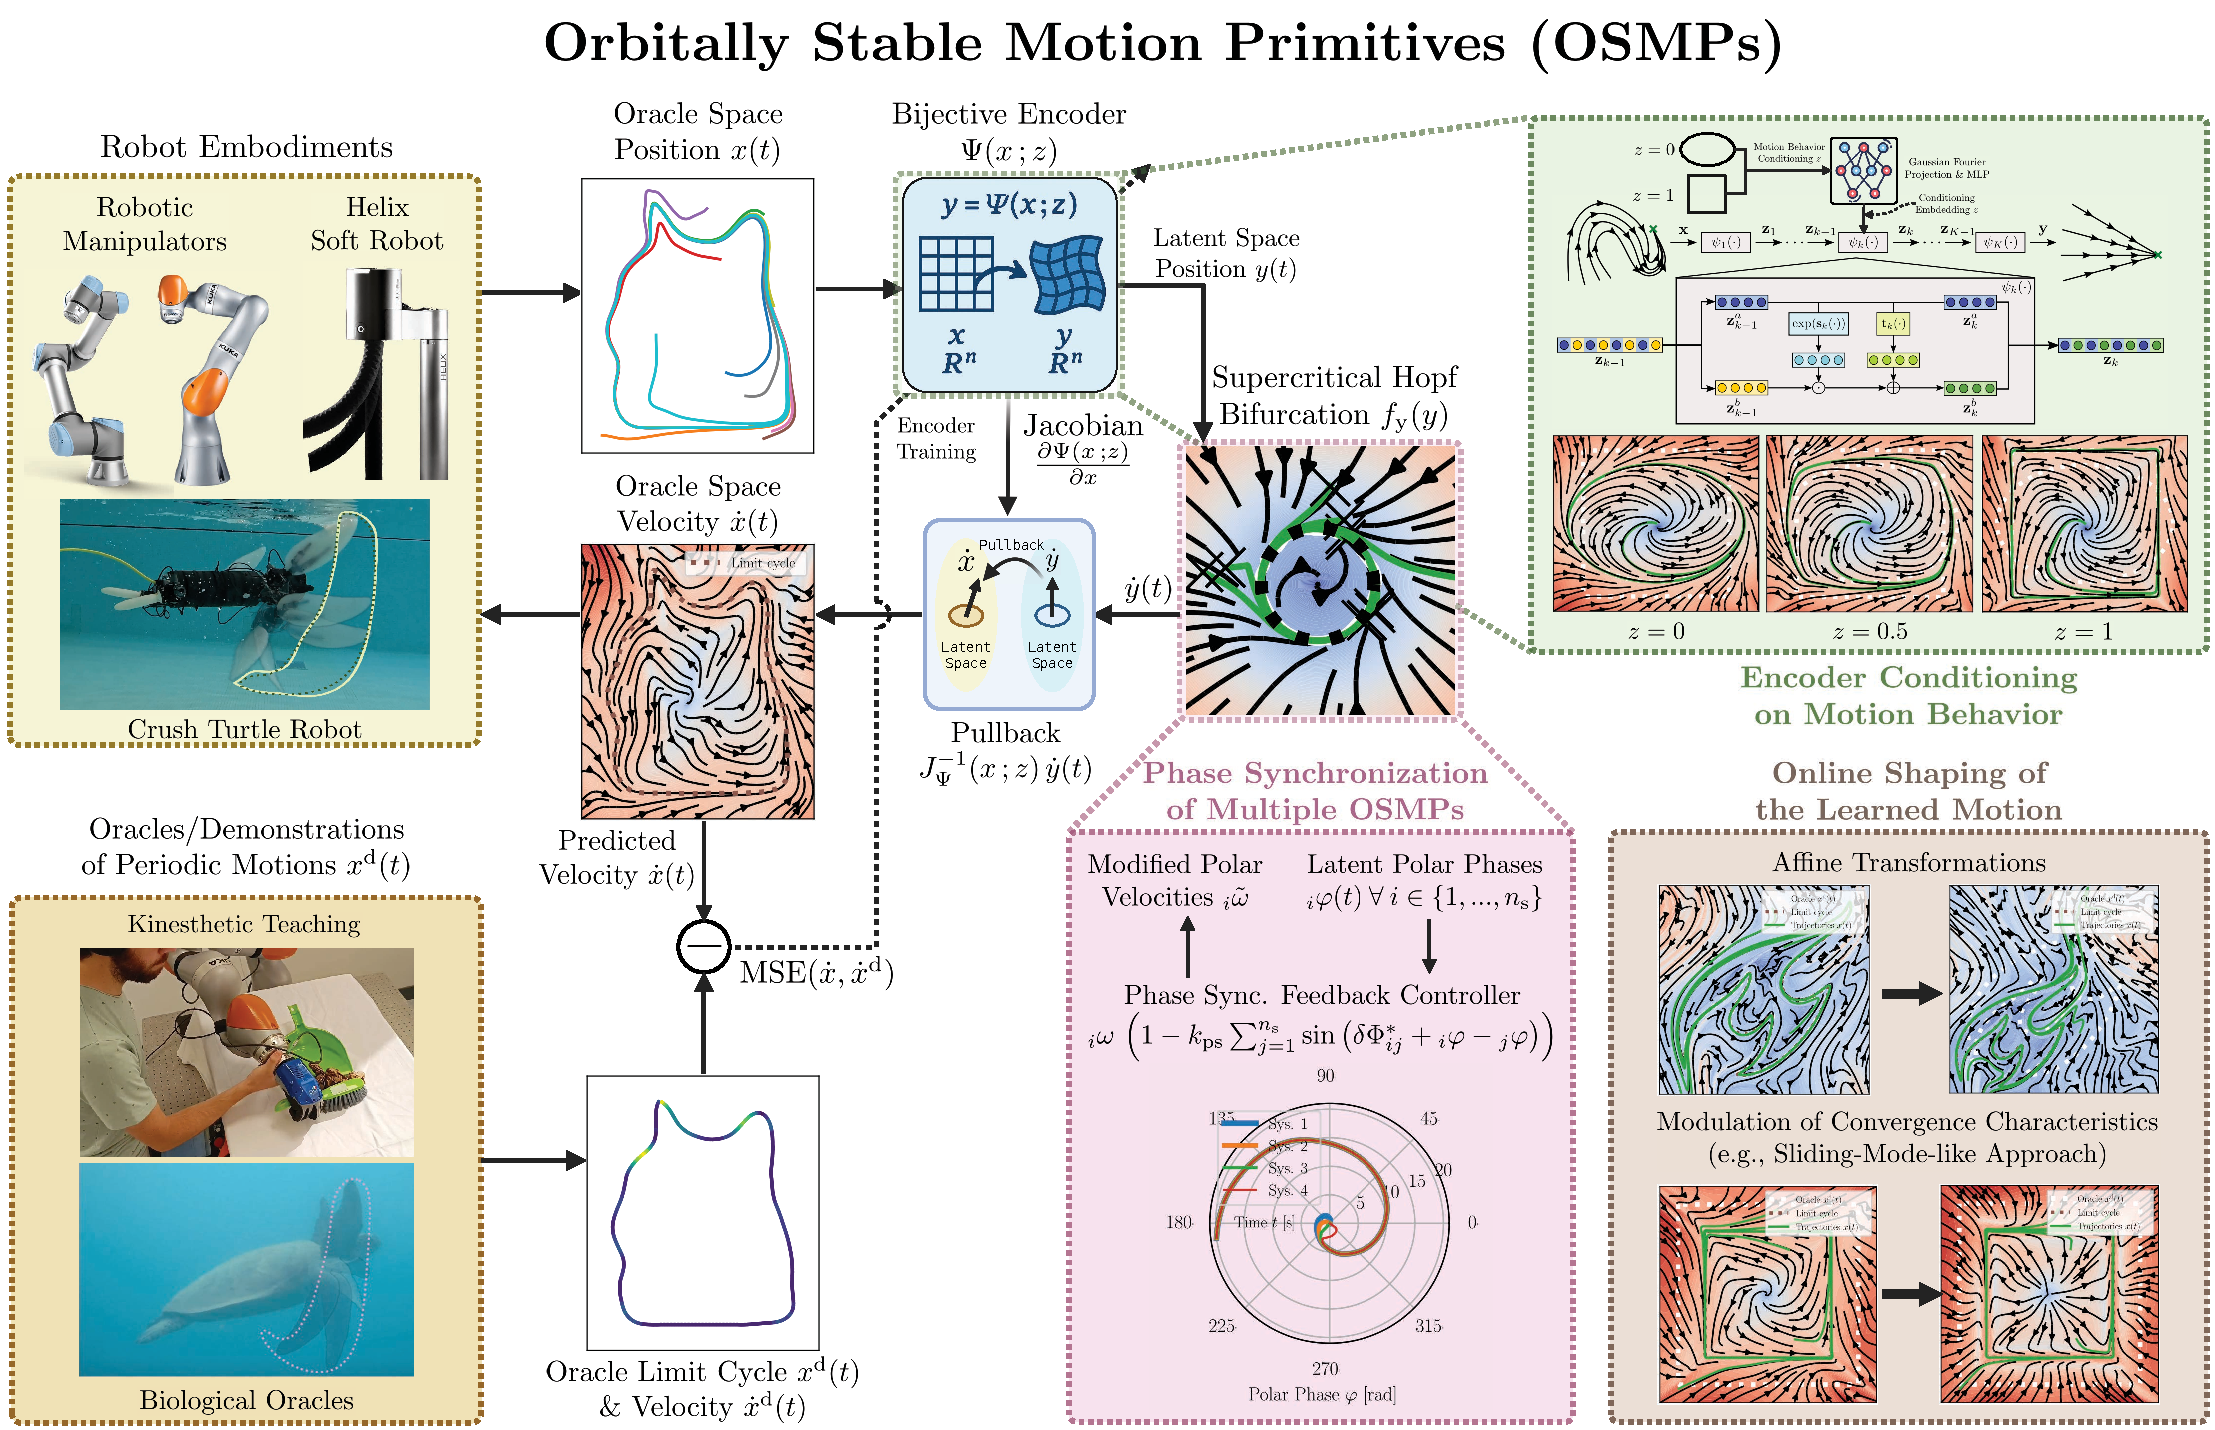
\includegraphics[width=1.0\linewidth]{osmp/figures/methodology_overview/osmp_methodology_overview_v3_compressed.pdf}
    % \includesvg[width=1.0\linewidth]{figures/methodology_overview/osmp_methodology_overview_v2.svg}
    \caption{
    \textbf{Methodology of \glspl{OSMP}.}
    Periodic motions can be learned from demonstration via a \gls{DMP} that combines a bijective encoder with latent space dynamics defined by a supercritical Hopf bifurcation. After encoding the current oracle space position of the system into latent space and predicting the latent space velocity, the pullback operator projects the velocity back into oracle space and represents a motion reference for the various robot embodiments. During training, we enforce both the predicted velocity and the exhibited limit cycle to match the demonstrations that are, for example, provided via kinesthetic teaching or based on biological oracles.
    Multiple contributions increase the practical usefulness of the proposed methods, which include a technique to synchronize multiple \glspl{OSMP} in phase, an approach to shape the learned motion online without requiring retraining via affine transformations or even modulating the convergence characteristics, and a methodology for conditioning the encoder on the oracle which allows the \gls{OSMP} to capture multiple distinct motion behaviors and even smoothly interpolate between them.
    The depiction of the Euclideanizing flows architecture is adapted from \citet{rana2020euclideanizing}.
    }
    \label{fig:osmp:methodology_overview}
\end{figure}

\begin{table}
    \centering
    % Captions go above tables
    \caption{\textbf{Comparison of characteristics of proposed methods against relevant baseline methods.} 
    In some cases, we denote with a \emph{x$^*$} that the feature could (probably) be developed for the respective method, but was not presented in the original paper.
    \emph{Note:} The CLF-CBF-NODE only guarantees convergence to a target trajectory as predicted by the learned NODE. However, the learned NODE is not guaranteed to exhibit a stable limit cycle behavior.
    }
    \label{tab:osmp:osmp_characteristics_vs_baselines} % give each table a logical label name
    \begin{scriptsize}
    \setlength\tabcolsep{2.0pt}
    \begin{tabular}{l ccccccc}\\
        \toprule
        \textbf{Method} & \textbf{Model} & \textbf{Orb. Stability} & \textbf{Velocity} & \textbf{$N$-Policies} & \textbf{Task} & \textbf{Smooth Task}\\
        & \textbf{Expressiveness} & \textbf{Guarantees} & \textbf{Imitation} & \textbf{Sync.} & \textbf{Conditioning} & \textbf{Interpolation}\\
        \midrule
        \gls{MLP} \& \gls{RNN} & Moderate & x & Noisy & x & $\checkmark$ & x\\
        \gls{NODE} & Moderate & x & $\checkmark$ & x & $\checkmark$ & x\\
        \gls{DP}~\citep{chi2023diffusion} & High & x & Noisy & x & $\checkmark$ & x\\
        Classical Rhythmic \glspl{DMP}  & Limited & $\checkmark$ & $\checkmark$ & $\checkmark$ & x & x\\
        HB-GMR~\citep{khadivar2021learning} & Limited & $\checkmark$ & x & x$^*$ & x & x\\
        Imitation Flow (iFlow)~\citep{urain2020imitationflow} & Moderate & $\checkmark$ &  $\checkmark$ & x$^*$ & x$^*$ & x\\
        CLF-CBF-NODE~\citep{nawaz2024learning} & Moderate & x & $\checkmark$ & x & x$^*$ & x\\
        \gls{SPDT}~\citep{zhi2024teaching} & Moderate & $\checkmark$ & x & x$^*$ & x & x\\
        \textbf{\gls{OSMP} (ours)} & Moderate & $\checkmark$ & $\checkmark$ & $\checkmark$ & $\checkmark$ & $\checkmark$\\
        \bottomrule
    \end{tabular}
    \end{scriptsize}
\end{table}